\documentclass[svgnames,11pt]{beamer}
\input{/home/tof/Documents/Cozy/latex-include/preambule_commun.tex}
\input{/home/tof/Documents/Cozy/latex-include/preambule_beamer.tex}
%\usepackage{pgfpages} \setbeameroption{show notes on second screen=left}
\author[]{Christophe Viroulaud}
\title{Exercices parcours graphe\\Correction}
\date{\framebox{\textbf{Algo 20}}}
%\logo{}
\institute{Terminale - NSI}

\begin{document}
\begin{frame}
\titlepage
\end{frame}
\section{Exercice 1}
\begin{frame}
    \frametitle{Exercice 1}

    \begin{center}
        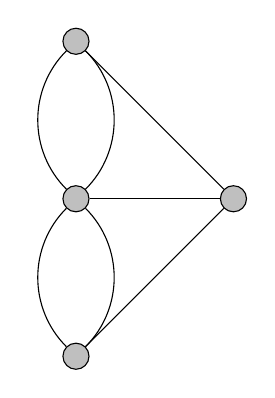
\begin{tikzpicture}
        \node[draw,circle,fill=gray!50] (A)at(0,2) {};
        \node[draw,circle,fill=gray!50] (B)at(0,0) {};
        \node[draw,circle,fill=gray!50] (C)at(0,-2) {};
        \node[draw,circle,fill=gray!50] (D)at(2,0) {};
        \draw[-,>=latex] (A) to[bend left=-45] (B);
        \draw[-,>=latex] (A) to[bend left=45] (B);
        \draw[-,>=latex] (C) to[bend left=-45] (B);
        \draw[-,>=latex] (C) to[bend left=45] (B);
        \draw[-,>=latex] (B) -- (D);
        \draw[-,>=latex] (A) -- (D);
        \draw[-,>=latex] (C) -- (D);
        \end{tikzpicture}
        \captionof{figure}{Les sept ponts de Königsberg}
        \label{graphe}
        \end{center}
Tous les sommets sont de degré impair. Il n'est pas possible de réaliser un cycle eulérien.
\end{frame}
\section{Exercice 2}
\begin{frame}
    \frametitle{Exercice 2}

    \begin{itemize}
        \item L'ordre est 8.
        \item Le degré de D est 4.
    \end{itemize}

\end{frame}
\begin{frame}[fragile]
    \frametitle{}

\begin{center}
\begin{lstlisting}[language=Python , basicstyle=\ttfamily\small, xleftmargin=2em, xrightmargin=2em]
graphe = {"A": ["B", "C", "D"],
    "B": ["A", "D", "E"],
    "C": ["A", "D", "F", "H"],
    "D": ["A", "B", "C", "G"],
    "E": ["B", "F"],
    "F": ["C", "E"],
    "G": ["D"],
    "H": ["C"]}
\end{lstlisting}
\end{center} 

\end{frame}
\begin{frame}[fragile]
    \frametitle{}

\begin{center}
\begin{lstlisting}[language=Python , basicstyle=\ttfamily\small, xleftmargin=0.2em, xrightmargin=0em]
def profondeur_dict(graphe: dict, noeud: str, visites: dict) -> None:
    if not visites[noeud]:
        print(noeud, end=" ")
        visites[noeud] = True
        for voisin in graphe[noeud]:
            profondeur_dict(graphe, voisin, visites)
\end{lstlisting}
\captionof{code}{Création de la fonction}

\begin{lstlisting}[language=Python , basicstyle=\ttfamily\small, xleftmargin=0.2em, xrightmargin=0em]
visites_dico = {chr(65+i): False for i in range(8)}
profondeur_dict(graphe, "A", visites_dico)
\end{lstlisting}
\captionof{code}{Appel de la fonction}
\end{center} 

\end{frame}
\begin{frame}[fragile]
    \frametitle{}

\begin{center}
\begin{lstlisting}[language=Python , basicstyle=\ttfamily\small, xleftmargin=2em, xrightmargin=2em]
def get_indice(sommet: str) -> int:
    return ord(sommet)-65
\end{lstlisting}
\end{center} 

\end{frame}
\begin{frame}[fragile]
    \frametitle{}

\begin{center}
\begin{lstlisting}[language=Python , basicstyle=\ttfamily\small, xleftmargin=0.2em, xrightmargin=0em]
def profondeur_tab(graphe: dict, noeud: str, visites: dict) -> None:
    ind = get_indice(noeud)
    if not visites[ind]:
        print(noeud, end=" ")
        visites[ind] = True
        for voisin in graphe[noeud]:
            profondeur_tab(graphe, voisin, visites)
\end{lstlisting}
\captionof{code}{Création de la fonction}

\begin{lstlisting}[language=Python , basicstyle=\ttfamily\small, xleftmargin=0.2em, xrightmargin=0em]
visites_tab = [False for i in range(8)]
profondeur_tab(graphe, "A", visites_tab)
\end{lstlisting}
\captionof{code}{Appel de la fonction}
\end{center} 

\end{frame}
\begin{frame}
    \frametitle{}

    \begin{aretenir}[Observation]
Les deux fonctions construites permettent de s'affranchir du coût de parcours du tableau \textbf{\texttt{visites}} à chaque appel récursif. En effet, la vérification de la valeur associée à une clé dans un dictionnaire ou celle de la lecture du booléen dans le tableau s'effectuent en temps constant.
    \end{aretenir}

\end{frame}
\section{Exercice 3}
\begin{frame}[fragile]
    \frametitle{Exercice 3}

\begin{center}
\begin{lstlisting}[language=Python , basicstyle=\ttfamily\small, xleftmargin=2em, xrightmargin=2em]
graphe = [
        [1, 2],
        [3],
        [5],
        [0, 2, 6],
        [1],
        [4],
        [],
        [2]]
\end{lstlisting}
\end{center}

\end{frame}
\begin{frame}[fragile]
    \frametitle{}

\begin{center}
\begin{lstlisting}[language=Python , basicstyle=\ttfamily\small, xleftmargin=0.2em, xrightmargin=-3em]
def dfs(graphe: list, sommet: int, visites: list) -> None:
    # en cours de parcours
    visites[sommet]["coul"] = GRIS
    for voisin in graphe[sommet]:
        # pour chaque voisin non encore atteint
        if visites[voisin]["coul"] == BLANC:
            visites[voisin]["pred"] = sommet
            dfs(graphe, voisin, visites)
    # parcours terminé pour ce sommet
    visites[sommet]["coul"] = NOIR
\end{lstlisting}
\end{center}
\begin{aretenir}[Remarque]
La vérification de la couleur s'effectue avant l'appel récursif (ligne 6) au lieu de se faire en début de fonction; ceci afin de ne modifier le prédécesseur qu'à la première visite.
\end{aretenir}
\end{frame}
\end{document}